\documentclass[11pt]{article}
\usepackage[margin=0.8in]{geometry}
\usepackage{amsmath,amssymb,graphicx,xurl,hyperref}
\hypersetup{colorlinks=true,urlcolor=blue}
\setlength{\parindent}{0pt}
\setlength{\parskip}{6pt}
\begin{document}
{\LARGE Actual affine Boolean contraction}\par
{\large Denominator clearing, integral local charts, and quotient transport}\par
November 9, 2026. Source commit \texttt{fa4e2bbab}.\par
Unsigned producer evidence throughout: [pcc:unverified].

\textbf{Result and assumptions.}
The actual source D.8 contraction admits denominator clearing with exponent
exactly $M$, the number of real row ports. The zero-output factor is affine;
its constant term must survive homogenization. For immutable $A(Y), B(X)$ and
$\ell_0(z)=1-z$, $\ell_1(z)=z$, put
\[
 F(W)=\sum_{X,Y\in\{0,1\}^M} A(Y)B(X)
       \prod_{j=1}^M\ell_{Y_j}((WX)_j).
\]
If $D$ is a common unit and $n_j=(NX)_j$, each factor clears as
\[
 D\ell_1(n_j/D)=n_j,\qquad
 D\ell_0(n_j/D)=D-n_j.
\]
Multiplying the $M$ factors and distributing both sums proves
\[
 D^M F(N/D)=\sum_{X,Y} A(Y)B(X)
       \prod_j\begin{cases}n_j&Y_j=1,\\D-n_j&Y_j=0.\end{cases}
\]
This is valid over every commutative ring, including rings with nilpotents.
The Lean proof imposes no $M>0$ restriction.

\textbf{Actual packed Cauchy repair.}
Set $L=2^a$, $N_{ij}=B_{ij}^2$ within a packet, and zero between packets;
$D=\sum_s B_s$. The imported actual $B_s$ has degree at most $2L-1$.
Each cleared factor therefore has degree at most $2(2L-1)$, giving
\[
 \deg\bigl(D^M F(N/D)\bigr)\leq 2M(2L-1).
\]
The polynomial statement is over any $\mathbb Q$-algebra with fixed $A,B$.
At rational points the clearing identity requires $D(T)\ne0$; there is no
cancellation at poles. An injective supplied placement gives $U(0)=I$ and
$F(U(0))=\sum_X A(X)B(X)$. Padding has no real ports. A packing constructor
and its cost are separate obligations.

\textbf{Controls.}
$3\ell_0(2/3)=1$, whereas $\ell_0(2)=-1$. The native identity certificate
\texttt{IDC1had86c2d70ea770ef} covers the polynomial rearrangement
$d(1-zi)=d-z(di)$; the unit relation is separately proved in Lean. The unchanged
native checker accepts extra evaluation points and rejects naive substitution
as a false identity. This finite-field check is supporting evidence, not the
quantified ring proof or an independent attestation.
\newpage
\textbf{Actual local series and finite quotients.}
The existing construction uses the concrete rational integral ring
$\mathcal O=\{q\in\mathbb Q:|q|_2\leq1\}$. At every source node it constructs
the shifted denominator series and an integral reciprocal with both inverse
identities. Packaging those actual series as a unit instantiates the affine
clearing theorem for the packet-restricted actual local kernel. Applying any
ring homomorphism transports the entire weighted identity. This includes
reduction by a finite jet ideal; arbitrary coefficient truncation is not
asserted to be a ring homomorphism.

\begin{center}
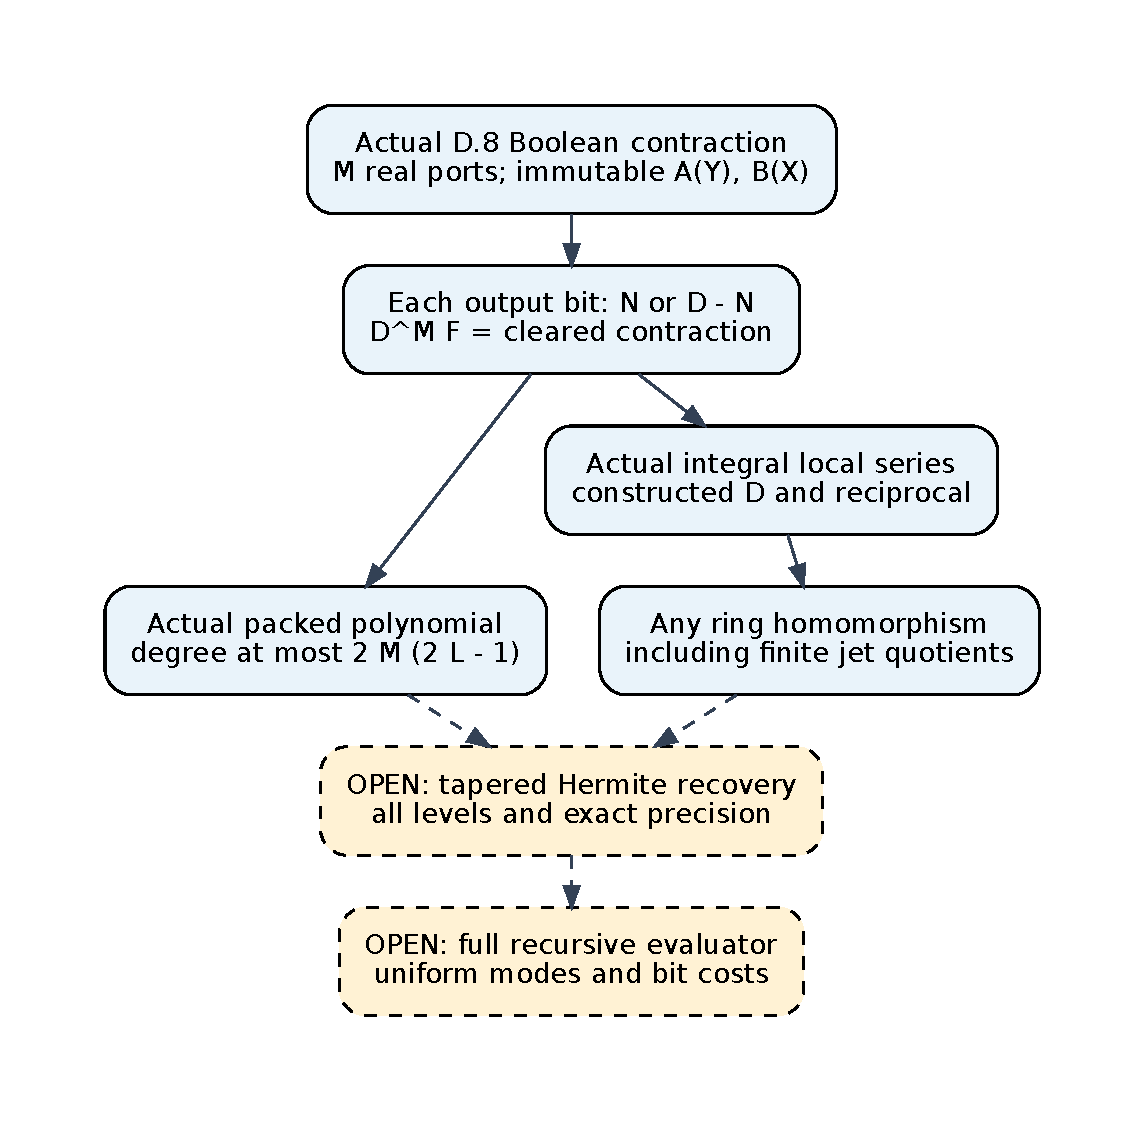
\includegraphics[width=0.88\textwidth,height=0.49\textheight,keepaspectratio]{bridge.pdf}
\end{center}
Solid boxes describe this proof component; dashed boxes remain open.

\textbf{Checks.}
Default build \texttt{packed-build-004.log} passed. The actual repository source
gate reports 140 declarations, no extra trusted axioms. Foundations are
\texttt{propext}, \texttt{Classical.choice}, \texttt{Quot.sound}. The official
import-inclusive fresh replay exited0; see
\path{lean/contraction-fresh-status.json} and its raw log. Failed elaborations
and the first native build are retained. No checker, trust policy, kernel or
dependency revision was changed. Native module tests: 22 passed, zero failed.
These are unsigned producer checks [pcc:unverified].

No timings or speedups are inferred from compiler logs. Historical comparison
plots and scoreboards are unchanged because no measured value or admitted
performance row changed.
\newpage
\textbf{Proof map.}
All names below are in \texttt{BooleanContraction} or \texttt{PackedContraction}.
The report Markdown and \path{lean/contraction-claim-pins.json} bind each name
and canonical statement hash to its unsigned PCC record.

\begin{tabular}{p{0.31\textwidth}p{0.61\textwidth}}
Affine weighted contraction & \texttt{sourceContractionClearing}, PCC-20261109-87aebd\\[5pt]
Actual rational point equality & \texttt{packedPointClearing}, PCC-20261109-205f61\\[5pt]
Mapped actual polynomial degree & \texttt{actualPackedContractionDegree}, PCC-20261109-21b592\\[5pt]
Origin under injective placement & \texttt{actualPackedOriginContraction}, PCC-20261109-7987a6\\[5pt]
Actual integral local identity & \texttt{actualLocalContractionClearing}, PCC-20261109-9e5d39\\[5pt]
Arbitrary ring-map transport & \texttt{mappedLocalContractionClearing}, PCC-20261109-055aa0
\end{tabular}

\textbf{Sources checked.}
The primary manuscript is OpenAI, \emph{The Exponential Time Hypothesis is False},
October 25, 2026, Appendix D.4.2--D.4.4, especially D.7--D.10. PDF SHA256:
\path{5b1612dc2eebb2cad5b4cbe62d1fed2982f01ab1908c26f70010a651487e8123}.
Pinned release:
\url{https://github.com/openai/math/blob/7ef5c0cc5ca4b0e072b7a050fca09ab24bc6fa3a/preprints/The-Exponential-Time-Hypothesis-is-False-October-25-2026/paper.pdf}.
Repository fallback review: common-kernel Boolean gauges, its
\texttt{GaugeCounterexample.lean}, and tensor-variants matched-level review.
The KB MCP is unavailable and wrapper status/search exited 127. This bounded
review does not establish novelty or survey exhaustion.

\textbf{Next discriminating obligation.}
Source D.5 uses $h=\lceil3M/u\rceil$ and
$q_t=h\max(0,u-v_2(t))$. The odd-node lower bound $Lhu\geq3ML$ alone does
not imply enough jets for doubled degree $2M(2L-1)$. Prove the total over
all active levels, then construct exact Hermite recovery with its finite
precision loss. The first-three-level numerical margin is useful evidence,
but is not that recovery theorem. Since $D(0)=1$, recovering the cleared value
recovers the target. Local construction and powering costs must be charged.

The explicit double sum is a correctness specification with exponentially
many assignments; it does not supply a faster evaluator. Uniform modes,
child-entry construction and complete recursive bit costs remain open.
The scalar repair still preserves the identity at the origin, so rank reduction
there requires a further mechanism.

\textbf{Reproduction.}
With pinned Lean 4.35.0 on PATH, from the repository root:
\begin{quote}\small\ttfamily
lake -d research/prime\_common\_scalar\_20261108/lean build\par
lake -d research/prime\_common\_scalar\_20261108/lean \textbackslash\par
\quad env leanchecker --fresh --verbose PackedContraction
\end{quote}
Native certificate reproduction commands and exact scope are in
\path{identity/README.md}. Sources and all logs are versioned alongside this report.
\end{document}
